% $Id: INF_Poster.tex 7714 2011-08-31 17:34:46Z tkren $
%
% TU Wien - Faculty of Informatics
% poster template
%
% This template is using the beamer document class and beamerposter package, see
% <http://www.ctan.org/tex-archive/macros/latex/contrib/beamer/>
% <http://www.ctan.org/tex-archive/macros/latex/contrib/beamerposter/>
% <http://www-i6.informatik.rwth-aachen.de/~dreuw/latexbeamerposter.php>
%
% For questions and comments send an email to
% Thomas Krennwallner <tkren@kr.tuwien.ac.at>
%

\PassOptionsToPackage{svgnames}{xcolor}

\documentclass[final,hyperref={pdfpagelabels=true}]{beamer}

\makeatletter
  \def\beamer@calltheme#1#2#3{%
    \def\beamer@themelist{#2}
    \@for\beamer@themename:=\beamer@themelist\do
    {\usepackage[{#1}]{\beamer@themelocation/#3\beamer@themename}}}

  \def\usefolder#1{
    \def\beamer@themelocation{#1}
  }
  \def\beamer@themelocation{}

\usefolder{style}

\usepackage{style/TUINFPST}
\usepackage{ragged2e}    %% provides \justifying
\usepackage{sidecap}     %% for images with side captions
\usepackage{wrapfig}
\usepackage[object=vectorian]{pgfornament} %%  http://altermundus.com/pages/tkz/ornament/index.html
\usepackage{tikz}
\usepackage{enumitem}

\title[Software Engineering \& Internet Computing]{Concurrent Programming with\\[.2\baselineskip]Actors and Microservices}
% if you have a long title looking squeezed on the poster, just force
% some distance:
% \title[Computational Intelligence]{%
%   Integration of Conjunctive Queries over \\[0.2\baselineskip]%
%   Description Logics into HEX-Programs %\\[0.2\baselineskip]%
% }
\author[max@irro.at]{Maximilian Irro}
\institute[]{%
  Technische Universit{\"a}t Wien\\[0.25\baselineskip]
  Institut f{\"u}r Information Systems Engineering\\[0.25\baselineskip]
  Arbeitsbereich: Compilers and Languages\\[0.25\baselineskip]
  Betreuer: Ao.Univ.Prof. Dipl.-Ing. Dr. Franz Puntigam
}
\titlegraphic{
\includegraphics[height=52mm]{complang-logo-neu}}
\date[\today]{\today}
\subject{epilog}
\keywords{concurrent programming, actor model, microservices}



%% A macro with two arguments to change ornaments and colors easily
%% Syntax -- \sectionlinetwo{<color>}{<ornament>}
\newcommand{\sectionlinetwo}[2]{%
  \nointerlineskip 
  \vspace{.5\baselineskip}
  \hspace{\fill}
  {\color{#1}
    \resizebox{0.3\linewidth}{3ex}
    {{%
    {\begin{tikzpicture}
    \node (C) at (0,0) {};
    \node (D) at (9,0) {};
    \path (C) to [ornament=#2] (D);
    \end{tikzpicture}}}}}%
    \hspace{\fill}
    \par\nointerlineskip \vspace{.5\baselineskip}
  }

%% Change the default (blueish-gray) color of description list terms
\setlist[description]{format=\color{Black}} 


%%%%%%%%%%%%%%%%%%%%%%%%%%%%%%%%%%%%%%%%%%%%%%%%%%%%%%%%%%%%%%%%%%%%%%%%%%%%%%%%%%%%%%
% Display a grid to help align images 
%\beamertemplategridbackground[1cm]

% for crop marks, uncomment the following line
%\usepackage[cross,width=88truecm,height=123truecm,center]{crop}

%%%%%%%%%%%%%%%%%%%%%%%%%%%%%%%%%%%%%%%%%%%%%%%%%%%%%%%%%%%%%%%%%%%%%%%%%%%%%%%%%%%%%%

\begin{document}

  % We have a single poster frame.
  \begin{frame}

    \newcommand{\lmodern}{\fontfamily{lmr}\selectfont}
    
    %\renewcommand\rmdefault{lmr}
    %\renewcommand\sfdefault{lmss}
    %\renewcommand\ttdefault{lmtt}

    %\renewcommand\rmdefault{lmr}
    %\renewcommand\sfdefault{lmss}
    %\renewcommand\ttdefault{lmtt}

    %\rmfamily % roman font family

    \vspace*{\baselineskip}

  \begin{columns}[t]
      \begin{column}{.04\textwidth}
        % intentionallyy left 
      \end{column}
      \begin{column}{.92\textwidth}

        \textsf{\textbf{INTRODUCTION}} \\
        \vspace*{.5\baselineskip}
        {\lmodern\justify
          \begin{justify}
          Concurrent programming manages multiple concerns simultaneously. This work fills a gap in the literature that emphasizes the connections between the \textbf{actor model} and the \textbf{microservice paradigm}. Both introduce concurrent computational units into software architectures. We investigate why actors and microservices qualify for programming concurrency and how they facilitate concurrent execution. We evaluate the expressive capabilities of actors and microservices and compare their performance relative to a non-trivial scenario of a concurrent system.
          \end{justify}
        }  

      \end{column}
      \begin{column}{.04\textwidth}
        % intentionallyy left 
      \end{column}
  \end{columns}

  \vspace*{3\baselineskip}

  \begin{columns}[t]
    \begin{column}{.04\textwidth}
      % intentionallyy left 
    \end{column}
    \begin{column}{.43\textwidth}
      \textsf{\textbf{ACTOR MODEL}} \\
      \vspace*{.5\baselineskip}
      {\lmodern
        \begin{justify}
        The actor model defines theoretically well-known constructs which support concurrent, parallel and distributed execution. Actors encapsulate state exclusively and communicate via asynchronous message passing. All actors live inside a runtime system that concurrently executes them. Actors are passive computational units, since they only react to messages. Exclusive state ownership and isolated message processing results in single-threaded semantics internally. Actors are therefore free of synchronization requirements.
        \end{justify}
      }
    \end{column}
    \begin{column}{.06\textwidth}
      % intentionallyy left 
    \end{column}
    \begin{column}{.43\textwidth}
      \textsf{\textbf{MICROSERVICE PARADIGM}} \\
      \vspace*{.5\baselineskip}
      {\lmodern
        \begin{justify}
        The microservice paradigm composes complex functionality through relatively small, independent, highly cohesive and loosely coupled executables. Every microservices is a dedicated operating system process. They communicate via light-weight, technology-neutral message passing channels. Microservices are executed by an operating system scheduler, which results in concurrency and parallelism. Network-based communication enables distribution. Microservices are active units and show behavior on their own accord.
        \end{justify}
      }
    \end{column}
    \begin{column}{.04\textwidth}
      % intentionallyy left 
    \end{column}
  \end{columns}

  \vspace*{1.5\baselineskip}
  %\hrule
  \sectionlinetwo{Black}{88}
  \vspace*{1.5\baselineskip}
  
  \begin{columns}[t]
    \begin{column}{.04\textwidth}
        % intentionallyy left 
      \end{column}
    \begin{column}{.43\textwidth}
      \textsf{\textbf{EXPRESSIVENESS \& CAPABILITIES}} \\
      \vspace*{.5\baselineskip}
      {\lmodern
        \begin{justify}
        Our evaluation shows that both models have the same expressive capabilities regarding concurrent programming concerns. Both models apply varying implementation strategies with different trade-offs. We focued our capability evaluations on four main concerns:
        \end{justify}
        
        \vspace*{\baselineskip}

        \renewcommand\sfdefault{lmss} % so the descriptions won't show Arial font

        \begin{description}
          \item[\textbf{\textsf{Encapsulation}}] 
          \begin{justify}
          Actors and microservices conceptually encapsulate state exclusively. Shared-memory environments threaten the isolation of state. Programmers must not expose mutable state through reference sharing among actors. The microservice paradigm forbids shared memory sections. Operating systems enforce strict memory boundaries among system processes.
          \end{justify}

          \vspace*{1.5\baselineskip}

          \item[\textbf{\textsf{Communication}}] 
          \begin{justify}
          Actors have an asynchronous messaging primitive. Additional communication abstractions build on top of this primitive, and are therefore at most semi-synchronous. Microservices are open for every technology-neutral, message passing communication channel in every interaction style.
          \end{justify}

          \vspace*{1.5\baselineskip}

          \item[\textbf{\textsf{Concurrent Execution}}] 
          \begin{justify}
          Actors and microservices encapsulate state exclusively and communicate solely through message passing semantics. These properties result in a temporal and spacial decoupling, which is the foundation for concurrent execution through an actor runtime or an operating system.
          \end{justify}

          \vspace*{1.5\baselineskip}

          \item[\textbf{\textsf{Scalability}}] 
          \begin{justify}
          The ability to scale is a major argument for using actors and microservices. The concurrent and parallel execution capabilities as well as message passing interaction lead to good vertical scalability. The distribution capabilities additionally enable horizontal scalability.
          \end{justify}
        \end{description}
        
      }
    \end{column}
    \begin{column}{.06\textwidth}
        % intentionallyy left 
      \end{column}
    \begin{column}{.43\textwidth}
      \textsf{\textbf{EFFICIENCY \& BENCHMARK}} \\
      \vspace*{.5\baselineskip}
      {\lmodern
        \begin{justify}
        %We evaluated the efficiency of the programming models. A domain-specific search engine architecture is a non-trivial example for a system with many concurrent processing opportunities.
        
        We evaluated the efficiency of the programming models with respect to a non-trivial scenario of a concurrent system. Our scenario is a domain-specific search engine, since the architecture provides many opportunities to facilitate concurrent processing. 

        \vspace*{1.4\baselineskip}
        
        The benchmark results below are for an actor-based and a microservices-based system implementation of this scenario. We used Akka as the actor system and built the microservices on the Spring framework.
        \end{justify}
      }

      \renewcommand\sfdefault{lmss} % so the descriptions won't show Arial font
      
      \begin{columns}[t]
        \begin{column}{.46\textwidth}
          \begin{center}
          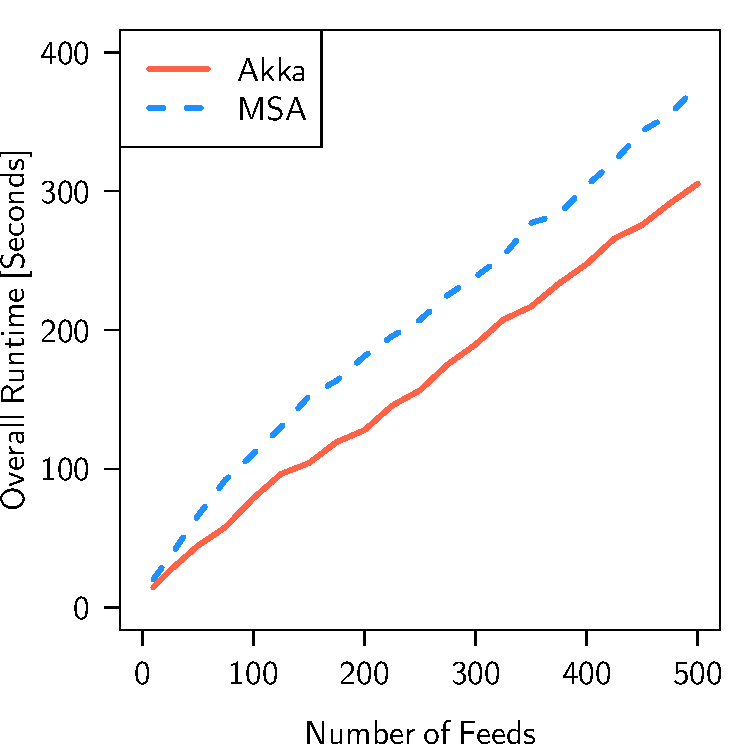
\includegraphics[width=1\textwidth]{graphics/eval-index-overall.pdf}
          \end{center}
        \end{column}
        \begin{column}{.08\textwidth}
          % Intentionally left blank
        \end{column}
        \begin{column}{.46\textwidth}
          {\lmodern
            \begin{justify}
              \textsf{\textbf{Experiment 1}} \\
              \vspace*{.5\baselineskip}
              The indexing phase facilitates asynchronous communication. The results show that the execution modality of actors is more efficient. Microservices have a higher runtime overhead, since they are separate system processes. 
            \end{justify}
          }
        \end{column}
      \end{columns}

      \vspace*{1.5\baselineskip}

      \begin{columns}[t]
        \begin{column}{.46\textwidth}
          \begin{center}
          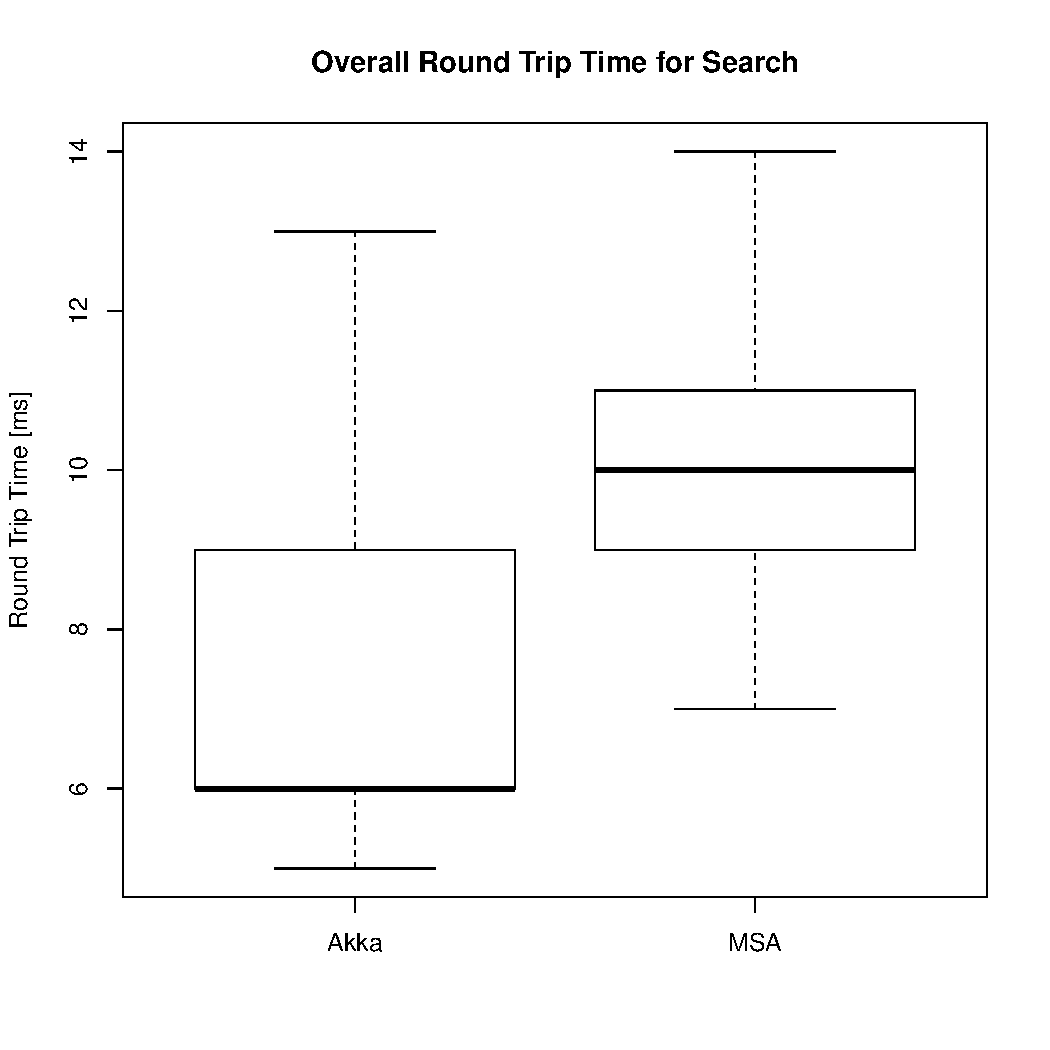
\includegraphics[width=1\textwidth]{graphics/eval-search-rtt-overall.pdf}
          \end{center}
        \end{column}
        \begin{column}{.08\textwidth}
          % Intentionally left blank
        \end{column}
        \begin{column}{.46\textwidth}
          {\lmodern\justify
            \begin{justify}
              \textsf{\textbf{Experiment 2}} \\
              \vspace*{.5\baselineskip}
              The time constraints of the retrieval phase favours synchronous interaction. Actors use a request/asynchronous response style. This semi-synchronous strategy shows better efficiency than strictly synchronous communication.  
            \end{justify}
          }
        \end{column}
      \end{columns}
    \end{column}
    \begin{column}{.04\textwidth}
        % intentionallyy left 
      \end{column}
  \end{columns}

\end{frame}

\end{document}

%%% Local Variables:
%%% TeX-PDF-mode: t
%%% TeX-debug-bad-boxes: t
%%% TeX-master: t
%%% TeX-parse-self: t
%%% TeX-auto-save: t
%%% reftex-plug-into-AUCTeX: t
%%% End:
